\documentclass[letterpaper]{report}
\usepackage[utf8]{inputenc}
\usepackage{csvsimple}
\usepackage[hidelinks]{hyperref}
\usepackage{graphicx}
\usepackage{float}
\usepackage{array}
\usepackage{longtable}
\usepackage{makecell}
% \usepackage{multirow}
% \usepackage{array, makecell}
\usepackage{adjustbox}
% \usepackage{showframe}
\usepackage{caption}
\usepackage{color}
\usepackage{listingsutf8}

% \usepackage{pstricks}
% \usepackage{auto-pst-pdf}
% \usepackage{pstricks-add}
% \usepackage{pst-eps}
\newcommand{\tabitem}{~~\llap{\textbullet}~~}

\definecolor{mygreen}{RGB}{154,255,77}
\definecolor{mygray}{gray}{0.5}
\definecolor{mylightgray}{gray}{0.95}
\definecolor{myblue}{RGB}{41,141,255}
\definecolor{myteal}{RGB}{0,150,136}

\lstset{
    language=SQL,
    backgroundcolor=\color{mylightgray},
    basicstyle=\scriptsize\ttfamily,
    keywordstyle=\color{myblue},
    commentstyle=\color{mygray},
    numberstyle=\color{mygreen},
    stringstyle=\color{myteal},
    numbers=left,
    numberstyle=\tiny\color{mygray},
    breaklines=true,
    breakatwhitespace=true,
    showstringspaces=false,
    tabsize=2,
    literate={{–}{\textendash}2
              {—}{\textemdash}2},
    inputencoding = utf8/latin1,  % Input encoding
    extendedchars = true,  % Extended ASCII
}

\title{
    \leavevmode{
\includegraphics[width=0.8\textwidth]{resources/Universita-degli-studi-di-torino-logo.png}\newline\newline}\\
    Progetto di Piattaforma di Home Booking \\
    \large Laboratorio Basi di Dati 2021/2022
}
\author{Eduard Antonovic Occhipinti, Iman Solaih, Marco Molica}

\begin{document}
\maketitle
\tableofcontents

\chapter{Progettazione Concettuale}
\section{Requisiti Iniziali}

Si vuole realizzare una base di dati per un servizio che permette di affittare e prenotare
alloggi di vario tipo ad esempio interi appartamenti, stanze private (camera privata e spazi
comuni) e stanze condivise (spazio in comune e camera condivisa).\newline
Gli utenti si registrano al servizio fornendo indirizzo email, password, nome, cognome,
numero o numeri di telefono. Se l’utente fornisce la foto della carta d’identità, viene
riconosciuto come verificato. Inoltre, l’utente deve indicare un metodo di pagamento per
poter prenotare. Gli utenti possono essere ospiti o “host” ovvero possono a loro volta
ospitare altri utenti del servizio in uno o più alloggi di loro proprietà. Inoltre gli “host” possono
diventare “superhost” se soddisfano i seguenti requisiti:
\begin{itemize}
    \item Devono aver completato almeno 10 soggiorni, per un totale di almeno 100 notti.
    \item Devono aver conservato un tasso di cancellazione dell'1\% (una cancellazione ogni
    100 prenotazioni) massimo.
    \item Devono aver mantenuto una valutazione complessiva di 4,8 \newline considerando tutti i
    soggiorni in tutte le case di sua proprietà.
\end{itemize}
Gli utenti superhost ricevono un badge sul loro profilo.
\newline
\newline
Gli alloggi sono descritti indicando un nome, l’indirizzo (visibile all’ospite solo quando la
prenotazione è confermata, altrimenti è visibile solo il comune), una descrizione, il prezzo per
notte per persona e i costi di pulizia, delle foto, i servizi (ad esempio, cucina, wi-fi, lavatrice,
ecc.), numero di letti e orario di check-in e check-out oltre all’host a cui appartiene, il rating
medio e il numero di recensioni (vedere Fig. 1).
\newline
\newline
Gli utenti possono aggiungere alcune case tra i preferiti. Gli utenti possono avere diverse
liste, ad esempio in base al viaggio che vogliono compiere.
\newline
\newline
Gli utenti possono prenotare degli alloggi di qualsiasi tipo indicando un intervallo di date per il
soggiorno e il numero degli ospiti. Se gli ospiti sono a loro volta utenti del servizio, se ne
possono indicare i nominativi. La prenotazione deve essere confermata o rifiutata dall’host.
La prenotazione ha un costo totale e se confermata viene eseguito il pagamento. Inoltre, la
prenotazione può essere cancellata sia dall’ospite che dall’host.
\newline
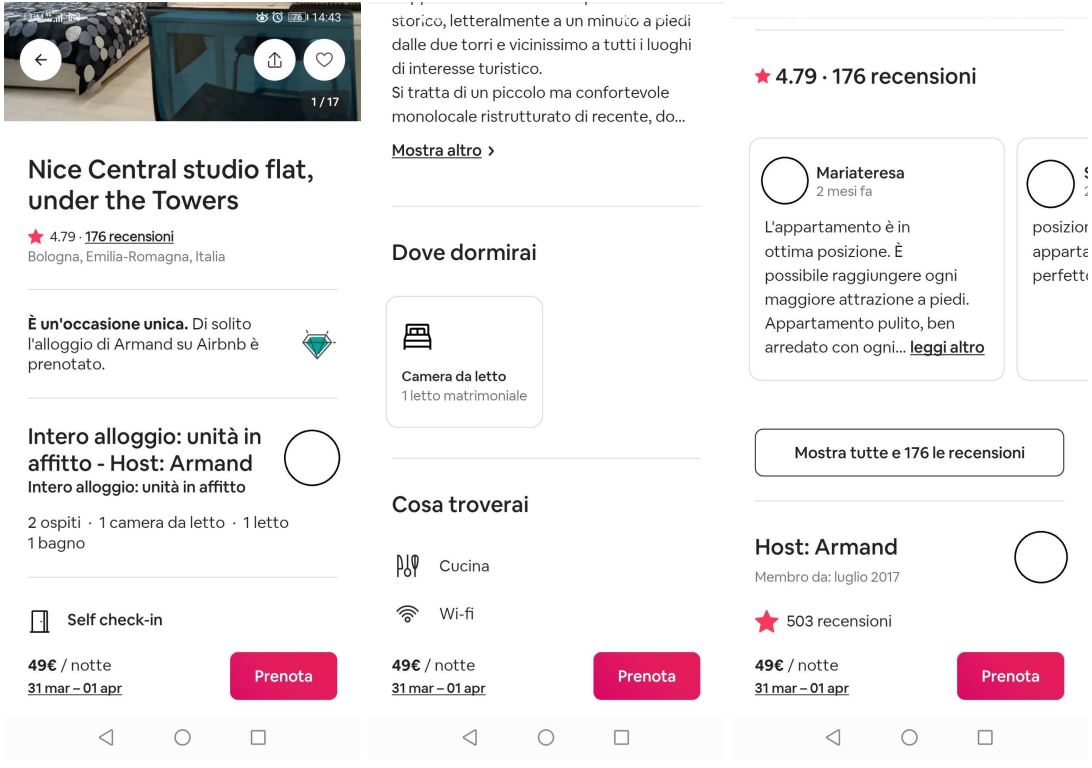
\includegraphics[width=\textwidth]{resources/airbnb.png}
\newline
Al termine del soggiorno, gli ospiti e gli host si possono valutare a vicenda. La recensione
fatta dagli ospiti comprende due testi (uno per l’appartamento e uno per l’host) e una serie di
punteggi in una scala da 1 a 5 su dimensioni come pulizia, comunicazione, posizione,
qualità/prezzo. La valutazione complessiva del soggiorno è una media delle valutazioni
ricevute sulle singole dimensioni. Le recensioni degli host comprendono solo un commento
testuale. Le recensioni possono essere visibili o non visibili. Diventano visibili quando
entrambi hanno fatto la recensione oppure se uno dei due non ha fatto la recensione, l’altra
diventa visibile dopo 7 giorni dalla fine del soggiorno. Gli host e gli ospiti possono
commentare più volte le review in cui sono coinvolti, creando un thread di discussione.
Le recensioni sono visibili sui profili degli utenti suddivise in base a quelle ricevute come
ospite e come host. La base di dati deve supportare le seguenti operazioni:
\begin{itemize}
    \item Una volta a settimana viene effettuato un calcolo per aggiornare il tasso di
    cancellazione di ciascun host.
    \item Una volta al giorno si controllano le condizioni per la qualifica di superhost e viene
    aggiornato lo status degli host.
    \item Una volta al mese viene calcolata la classifica degli alloggi più graditi.
\end{itemize}


\section{Glossario dei Termini}
\small
\setlength\extrarowheight{2pt}
\begin{tabular}{|l|p{4.95cm}|l|l|}
    \hline\bfseries Termine & \bfseries Descrizione                                                                                                                              & \bfseries Sinonimi                 & \bfseries Collegamenti                                              \\\hline
    Utente                  & Individuo che usufruisce del servizio. Può essere ospitato da altri utenti. Può caricare una carta di identità per diventare un profilo verificato & {Ospite}                           & \makecell[tl]{Host\\Prenotazione\\Recensione\\Liste\\Commento}      \\\hline
    Host                    & Utente che offre un servizio ovvero può ospitare altri utenti. Può diventare un superhost soddisfando determinati requisiti                        &                                    & \makecell[tl]{Utente\\Alloggio\\Prenotazione\\Recensione\\Commento} \\\hline
    Soggiorno               & {Utilizzo del servizio da parte di uno o più utenti, con durata variabile}                                                                         &                                    & \makecell[tl]{Prenotazione\\Alloggio}                               \\\hline
    Prenotazione            & Richiesta di soggiorno                                                                                                                             &                                    & \makecell[tl]{Alloggio\\Host\\Ospite}                               \\\hline
    Alloggio                & Proprietà posseduta da un utente. Può essere di diversi tipi                                                                                       & \makecell[tl]{Casa\\Struttura}     & \makecell[tl]{Prenotazione\\Liste\\Recensione}                      \\\hline
    Recensione              & Feedback lasciate tra gli utenti verso altri utenti o proprietà.Comprendono valutazioni e commenti testuali                                        & Review                             & \makecell[tl]{Utente\\Commento}                                     \\\hline
    Liste                   & Insiemi di alloggi preferiti da un utente                                                                                                          &                                    & \makecell[tl]{Alloggi\\Utente}                                      \\\hline
    Commento                & Descrizione testuale appartenente a una recenzione. Più commenti formano un thread                                                                 &                                    & \makecell[tl]{Recensione\\Utente}                                   \\\hline
    Servizio                & Funzionalità messa a disposizione dall'alloggio                                                                                                    &                                    & \makecell[tl]{Alloggio}                                             \\\hline
\end{tabular}
\normalsize
\newpage

\section{Requisiti rivisti e strutturati in gruppi di frasi omogenee}
\subsection{Requisiti rivisti}
Si vuole realizzare una base di dati per un servizio che permette di affittare e prenotare
alloggi di vario tipo ad esempio interi appartamenti, stanze private.
\newline
\newline
Per il dato utente registriamo: indirizzo email, password, nome, cognome, numeri di telefono, carta di identità, metodo di pagamento.
\newline
\newline
Per il dato host registriamo: superhost.
\newline
\newline
Per il dato soggiorno registriamo: data inizio, data fine, idalloggio, idprenotazione.
Ogni utente può avere 0 o più soggiorni.
\newline
\newline
Per il dato alloggio registriamo: nome, indirizzo, comune, descrizione, costo per notte per  persona, costo pulizia, numero di letti, orario check-in, orario check-out, rating medio(?)
Ogni host può possedere uno o più alloggi. Ad ogni alloggio sono associate 0 o più foto. Ogni alloggio offre 0 o più servizi. Per ogni alloggio sono scritte 0 o più recensioni.
\newline
\newline
Gli host per diventare superhost devono soddisfare i  seguenti requisiti:
\begin{itemize}
    \item Devono aver completato almeno 10 soggiorni, per un totale di almeno 100 notti.
    \item Devono aver conservato un tasso di cancellazione dell'1\% 
    (una cancellazione ogni 100 prenotazioni) massimo.
    \item Devono aver mantenuto una valutazione complessiva di 4,8 considerando 
    tutti i soggiorni in tutte le case di sua proprietà
\end{itemize}
Ogni utente può aggiungere 0 o più alloggi tra i preferiti e creare 0 più liste.
Per il dato lista registriamo: descrizione, nome
\newline
\newline
Per il dato prenotazione registriamo: costo prenotazione, idalloggio, stato, numero ospiti, id metodo di pagamento. Ogni prenotazione sarà associata ad un utente ed un host, potrà avere 0 o più ospiti associati. La prenotazione può essere cancellata sia dall'ospite che dall'host: verrà aggiornato lo stato.
\newline
\newline
Al termine del soggiorno, gli ospiti e gli host si possono valutare a vicenda. 
Per il dato recensione registriamo: visibilità, data, idautore, idutente, 
idalloggio, testo, valutazione pulizia, valutazione comunicazione, valutazione 
posizione, valutazione qualità-prezzo.
\newline
\newline
Le recensioni possono essere visibili o non visibili. Diventano visibili quando
entrambi hanno fatto la recensione oppure se uno dei due non ha fatto la recensione, l’altra
diventa visibile dopo 7 giorni dalla fine del soggiorno
\newline
\newline
Per il dato commento registriamo: idautore, testo, idrecensione
Gli host e gli ospiti possono commentare più volte le review in cui sono coinvolti, 
creando un thread di discussione.
\newline
\newline
Il sistema deve supportare le seguenti operazioni:
\begin{itemize}
    \item Una volta a settimana viene effettuato un calcolo per aggiornare 
    il tasso di cancellazione di ciascun host.
    \item Una volta al giorno si controllano le condizioni per la qualifica di 
    superhost e viene aggiornato lo status degli host.
    \item Una volta al mese viene calcolata la classifica degli alloggi più graditi
\end{itemize}

\subsection{Requisiti strutturati in gruppi di frasi omogenee}
\textbf{Frasi relative a utenti}:
\begin{itemize}
    \item Ogni utente può essere sia ospite di altri utenti che host.
    \item Gli utenti sono rappresentati da un nome, cognome, email, password e uno o più numeri di telefono
    \item Gli utenti possono memorizzare la foto della carta di identità,necessaria per essere considerati utenti verificati
    \item Gli utenti possono memorizzare zero o più metodi di pagamento. Per poter effettuare delle prenotazioni è necessario avere almeno un metodo di pagamento
    \item Gli utenti possono scrivere recensioni con valutazioni verso gli host e gli alloggi
    \item Gli utenti possono ricevere recensioni dagli host dopo un soggiorno
    \item Ogni utente può creare delle liste, in cui aggiungere gli alloggi preferiti
    \item Ogni utente può effettuare una o più prenotazioni, purchè abbia un metodo di pagamento. Può confermare o cancellare le proprie prenotazioni
    \item Ogni utente che ha effettuato una prenotazione, può aggiungere altri utenti ad essa, se registrati al servizio
    \item Ogni utente può scrivere commenti nei thread delle recensioni in cui è incluso \\
\end{itemize}
\bigskip
\textbf{Frasi relative a host}:
\begin{itemize}
    \item Un host è una specializzazione di utente, che può ospitare altri utenti.
    \item Un host può registrare uno o più alloggi
    \item Un host può scrivere recensioni testuali verso gli utenti che hanno effettuato un soggiorno presso i propri alloggi
    \item Un host può diventare un superhost se soddisfa determinati requisiti:
    \begin{itemize}
        \item Ha completato almeno 10 soggiorni, per un totale di almeno 100 notti
        \item Ha conservato un tasso di cancellazione dell'1%
        \item Ha mantenuto una valutazione complessiva di 4.8 tra tutti i soggiorni di tutti i suoi alloggi
    \end{itemize}
    \item Un host può cancellare o confermare una prenotazione ricevuta
\end{itemize}
\bigskip
\textbf{Frasi relative a soggiorno}:
\begin{itemize}
    \item Ogni soggiorno viene effettuato al seguito di una prenotazione confermata.
    \item Ogni soggiorno è caratterizzato da una data inizio e una data fine
    \item Ogni soggiorno viene effettuato in un alloggio, da uno o più utenti
    \item Per ogni soggiorno è richiesta una prenotazione
    \item Ogni soggiorno può ricevere una recensione, con valutazione
    \item La valutazione complessiva di un soggiorno è la media delle sue valutazioni
\end{itemize}
\bigskip
\textbf{Frasi relative a prenotazione}:
\begin{itemize}
    \item Ogni prenotazione è associata ad un alloggio
    \item Ogni prenotazione è caratterizzata da un costo totale, una data di prenotazione, una data di inizio, una data di fine
    \item Ogni prenotazione deve essere confermata o rifiutata dagli host
    \item Può essere cancellata dagli utenti o dagli host
    \item Non è possibile effettuare una prenotazione se l'utente non ha caricato un metodo di pagamento
    \item Quando confermata viene eseguito il pagamento
    \item Ogni prenotazione confermata è associata ad un soggiorno \\
\end{itemize}
\bigskip
\textbf{Frasi relative a Alloggio}:
\begin{itemize}
    \item Ogni alloggio è caratterizzato da un nome, un comune, un indirizzo, un costo per notte per persona, un costo pulizia, un numero di letti, orario del check-in, orario del check-out
    \item Ogni alloggio può avere 0 o più recensioni
    \item Ogni alloggio deve appartenere ad un host
    \item Più alloggi possono appartenere allo stesso host
    \item Un alloggio può essere di diversi tipo: intero appartamento, stanza privata o stanza condivisa
    \item Un alloggio di tipo stanza condivisa può ricevere prenotazioni per la stessa data fino al raggiungimento del numero di letti
    \item Un alloggio di tipo stanza privata o appartamento non può ricevere più prenotazioni per la stessa data
    \item Un alloggio può avere una o più foto
    \item Un alloggio può riceve delle recensioni
    \item La valutazione complessiva di un alloggio è la media delle valutazioni ricevute
    \item Un alloggio può essere aggiunto tra i preferiti di zero o più utenti
    \item Un alloggio può offire zero o più servizi
\end{itemize}
\bigskip
\textbf{Frasi relative a Recensione}:
\begin{itemize}
    \item Ogni recensione è caratterizzata da un corpo, una data e delle valutazioni
    \item Ogni recensione è associata ad un soggiorno
    \item Le recensioni sono di 3 tipi: fatte ad host, fatte ad utenti e fatte ad alloggio
    \item Una recensione su alloggio può contenere una valutazione della pulizia, una valutazione della posizione e una valutazione sul rapporto qualità-prezzo
    \item Una recensione su host può contenere una valutazione sulla comunicazione
    \item Una recensione su utenti non contiene valutazioni
    \item Ad ogni recensione può essere associato un thread di commenti
    \item Una recensione può essere lasciata da un host o da un utente
    \item Una recensione può essere visibile o non visibile
    \item Una recensione diventa visibile se sia l'autore che il recensito hanno pubblicato una recensione
    \item Una recensione diventa automaticamente visibile dopo 7 giorni dalla fine del soggiorno a cui è associata
\end{itemize}
\bigskip
\textbf{Frasi relative a Liste}:
\begin{itemize}
    \item Ogni lista è caratterizzata da un nome e una descrizione
    \item Una lista può contenere zero o più alloggi preferiti di un utente
    \item Ogni lista appartiene ad un solo utente
\end{itemize}
\bigskip
\textbf{Frasi relative a Commento}:
\begin{itemize}
    \item Ogni commento è caratterizzato da un testo
    \item Ogni commento può essere scritto nel thread di una recensione
    \item Ogni commento può essere scritto solo dall'utente o dall'host coinvolti nella recensione
\end{itemize}


\newpage
\section{Schema E-R + Business Rules}
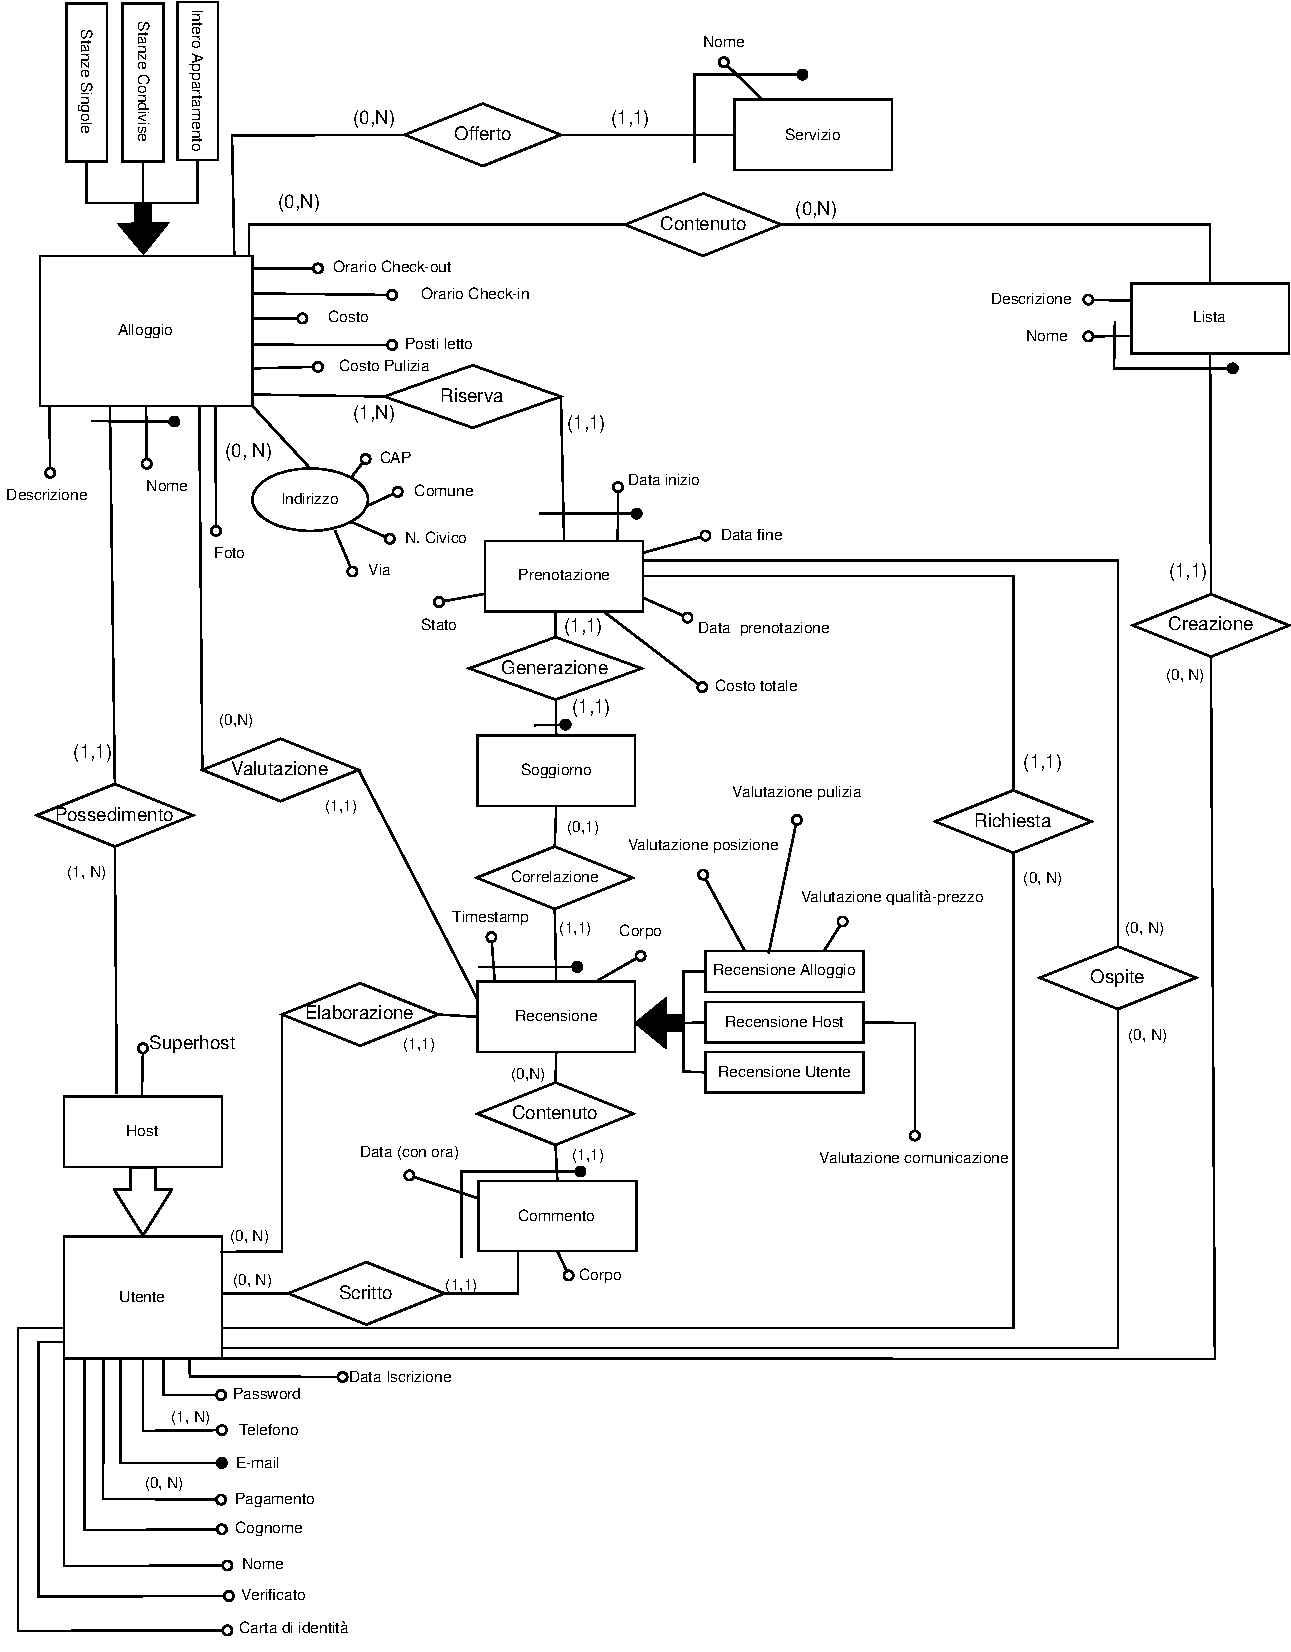
\includegraphics[width=\textwidth]{resources/pdf/ER.pdf}

\chapter{Progettazione Logica}
\section{Tavola dei Volumi}
\small
\setlength\extrarowheight{2pt}
\begin{longtable}{|l|c|c|p{6.2cm}|}
    \hline \textbf{Concetto} & \textbf{Tipo} & \textbf{Volume} & \textbf{Motivazione}                                                                                                                         \\\hline
    \endfirsthead

    \hline \textbf{Concetto} & \textbf{Tipo} & \textbf{Volume} & \textbf{Motivazione}                                                                                                                         \\\hline
    \endhead

    \hline \multicolumn{4}{|r|}{{Continua all pagina successiva}}                                                                                                                                             \\\hline
    \endfoot

    \hline
    \endlastfoot
    Utente                   & E             & 30.000.000      & {Ipotizziamo una piattaforma in cui sono iscritte 30 milioni di utenti}                                                                      \\\hline
    Host                     & E             & 150.000         & {Ipotizziamo che sulla piattaforma si iscriveranno circa 150 mila host}                                                                      \\\hline
    Alloggio                 & E             & 169.000         & {Ipotizziamo che nella piattaforma verranno registrati circa 169 mila alloggi}                                                               \\\hline
    Prenotazione             & E             & 36.000.000      & {Ipotizziamo che sulla piattaforma siano state effettuate circa 36 milioni di prenotazioni}                                                  \\\hline
    Soggiorno                & E             & 34.920.000      & {Ipotizziamo che sulla piattaforma ci siano stati circa 35 milioni di soggiorni}                                                             \\\hline
    Recensione               & E             & 12.000.000      & {Ipotizziamo che sulla piattaforma vengano scritte circa 12 milioni di recensioni}                                                           \\\hline
    Commento                 & E             & 16.000.000      & {Ipotizziamo che sulla piattaforma vengano scritti circa 16 milioni di commenti}                                                             \\\hline
    Lista                    & E             & 45.000.000      & {Ipotizziamo che sulla piattaforma vengano create circa 45 milioni di liste di alloggi preferiti}                                            \\\hline
    Servizio                 & E             & 20              & {Ipotizziamo che sulla piattaforma vengano messi a disposizione circa 20 servizi differenti}                                                 \\\hline
    Possedimento             & R             & 169.000         & {Ipotizziamo che nella piattaforma ogni host abbia almeno un alloggio, e che 1 host su 8 abbia 2-3 alloggi}                                  \\\hline
    Richiesta                & R             & 36.000.000      & {Ipotizziamo che nella piattaforma 4 utenti registrati su 5 abbiano fatto almeno una prenotazione, e 1 su 5 ne abbia fatto almeno 3}         \\\hline
    Generazione              & R             & 34.920.000      & {Ipotizziamo che sul totale delle prenotazioni, circa il 2\% vengano cancellate. Tutte le altre diventano soggiorni effettivi}               \\\hline
    Elaborazione             & R             & 12.000.000      & {Ipotizziamo che 1 utente su 3 che ha effettuato una prenotazione poi scriva una recensione}                                                 \\\hline
    Contenuto                & R             & 16.000.000      & {Ipotizziamo che circa 1 recensione su 3 abbia un thread con almeno 3 commenti e 1 su 3 abbia un solo commento}                              \\\hline
    Creazione                & R             & 45.000.000      & {Ipotizziamo che circa 6 utenti su 10 creino delle liste, con una media di 2-3 liste per ciascuno di questi utenti}                          \\\hline
    Scritto                  & R             & 16.000.000      & {Ipotizziamo che circa 1 utente su 5 abbia scritto un commento, e di questi uno ne abbia scritto circa 2-3}                                  \\\hline
    Correlazione             & R             & 12.000.000      & {Ipotizziamo che circa 1 soggiorno su 6 riceva una recensione da parte dell'utente o dell'host, e che 1 su 6 la riceva da parte di entrambi} \\\hline
    Riserva                  & R             & 36.000.000      & {Ipotizziamo che tutti gli alloggi vengano riservati circa 36 milioni di volte, una volta per ogni prenotazione}                             \\\hline
    Offerto                  & R             & 250.000         & {Ipotizziamo che ogni alloggio offra più di una decina di servizi}                                                                           \\\hline
    Valutazione              & R             & 2.000.000       & {Ipotizziamo che circa 1 recensione su 3 viene scritta verso un alloggio}                                                                    \\\hline
\end{longtable}
\normalsize 


\section{Tavola delle Operazioni}
\setlength\extrarowheight{2pt}
\small
\begin{longtable}{|c|p{3cm}|c|c|p{4.18cm}|}
    \hline \# & \textbf{Operazione}                                                                         & \textbf{Tipo} & \textbf{Frequenza} & \textbf{Motivazione}                                                                                                                                     \\\hline
    \endfirsthead

    \hline \# & \textbf{Operazione}                                                                         & \textbf{Tipo} & \textbf{Frequenza} & \textbf{Motivazione}                                                                                                                                     \\\hline
    \endhead

    \hline \multicolumn{5}{|r|}{{Continua alla pagina successiva}}                                                                                                                                                                                                                                          \\\hline
    \endfoot

    \hline
    \endlastfoot
    1         & Registrazione al servizio                                                                   & {I}           & 50.000/day         & Operazione iniziale della piattaforma che permette ad una persona di utilizzare il servizio                                                              \\\hline
    2         & Prenotazione di un alloggio                                                                 & {I}           & 25.000/day         & Operazione principale che permette di effettuare un soggiorno                                                                                            \\\hline
    3         & Conferma di una prenotazione                                                                & {I}           & 24.500/day         & {Operazione che permette di finalizzare la richiesta di una prenotazione, effettuando il pagamanto}                                                      \\\hline
    4         & Declino di una prenotazione                                                                 & {I}           & 500/day            & Operazione che permette di rifutare una prenotazione richiesta                                                                                           \\\hline
    5         & Scrittura di una recensione                                                                 & {I}           & 8000/day           & {Operazione che permette di lasciare un feedback testuale da parte di un host e/o di un utente, e una valutazione da parte di un utente}                 \\\hline
    6         & Scrittura di un commento                                                                    & {I}           & 13000/day          & {Operazione che permette ad un host e/o un utente di lasciare ulteriori feedback testuali ad una recensione}                                             \\\hline
    7         & Creazione di una lista di alloggi preferiti                                                 & {I}           & 7000/day           & Operazione che permette di creare dei raggruppamenti di alloggi preferiti                                                                                \\\hline
    8         & Registrazione di un nuovo alloggio                                                          & {I}           & 300/day            & Operazione che permette di inserire un nuovo alloggio nella piattaforma                                                                                  \\\hline
    9         & Aggiornamento del tasso di cancellazione di ciascun host                                    & {B}           & 1/week             & Operazione che una volta a settimana aggiorna il numero di prenotazioni cancellate da parte dell'host                                                    \\\hline
    10        & Calcolo del numero di soggiorni e tempo di soggiorno complessivo per ciascun host           & {B}           & 1/day              & {Operazione che permette di aggiornare il tempo e il numero di soggiorni complessivi per ogni host, in modo da poterne calcolare lo status di superhost} \\\hline
    11        & Calcolo della valutazione complessiva di ogni host per i soggiorni totali ai propri alloggi & {B}           & 1/day              & {Operazione che permette di aggiornare la media delle valutazioni ricevute per ogni host, in modo da poterne calcolare lo status di superhost}           \\\hline
    12        & Aggiornamento dello status di ciascun host                                                  & {B}           & 1/day              & Operazione che tenendo conto di altri calcoli effettua un aggiornamento per definire quali host sono considerati superhost                               \\\hline
    13        & Aggiornamento della classifica degli alloggi più graditi                                    & {B}           & 1/month            & Operazione che permette di ottenere gli alloggi con una valutazione media più alta                                                                       \\\hline
    14        & Aggiornamento della visibilità delle recensioni                                             & {B}           & 1/day              & Operazione che permette di aggiornare lo status di visibilità delle recensioni                                                                           \\\hline
\end{longtable}
\normalsize


\section{Ristrutturazione dello schema E-R}
\subsection{Analisi delle ridondanze}
\subsubsection{ridondanza 1}
All'interno dello schema ER è stata identificata 1 ridondanza: la relazione valutazione tra le entità alloggio e recensione. Questa ridondanza ci permette di ottenere le recensioni effettuate su un alloggio utilizzando solamente le entità alloggio e recensione.
La sezione della tavola dei volumi di interesse è:

\small
\setlength\extrarowheight{2pt}
\begin{longtable}{|l|c|c|p{6.3cm}|}
    \hline \textbf{Concetto} & \textbf{Tipo} & \textbf{Volume} & \textbf{Motivazione}                                                                                                                         \\\hline
    \endfirsthead

    \hline \textbf{Concetto} & \textbf{Tipo} & \textbf{Volume} & \textbf{Motivazione}                                                                                                                         \\\hline
    \endhead

    % \hline \multicolumn{4}{|r|}{{Continua all pagina successiva}}                                                                                                                                             \\\hline
    \endfoot

    \endlastfoot
    Alloggio                 & E             & 169.000         & {Ipotizziamo che nella piattaforma verranno registrati circa 169 mila alloggi}                                                               \\\hline
    Prenotazione             & E             & 36.000.000      & {Ipotizziamo che sulla piattaforma siano state effettuate circa 36 milioni di prenotazioni}                                                  \\\hline
    Soggiorno                & E             & 34.920.000      & {Ipotizziamo che sulla piattaforma ci siano stati circa 35 milioni di soggiorni}                                                             \\\hline
    Recensione               & E             & 12.000.000      & {Ipotizziamo che sulla piattaforma vengano scritte circa 12 milioni di recensioni}                                                           \\\hline
    Generazione              & R             & 34.920.000      & {Ipotizziamo che sul totale delle prenotazioni, circa il 2\% vengano cancellate. Tutte le altre diventano soggiorni effettivi}               \\\hline
    Correlazione             & R             & 12.000.000      & {Ipotizziamo che circa 1 soggiorno su 6 riceva una recensione da parte dell'utente o dell'host, e che 1 su 6 la riceva da parte di entrambi} \\\hline
    Riserva                  & R             & 36.000.000      & {Ipotizziamo che tutti gli alloggi vengano riservati circa 36 milioni di volte, una volta per ogni prenotazione}                             \\\hline
    Valutazione              & R             & 2.000.000       & {Ipotizziamo che circa 1 recensione su 3 viene scritta verso un alloggio}                                                                    \\\hline
\end{longtable}
\normalsize

\subsubsection{todo:titoletto}
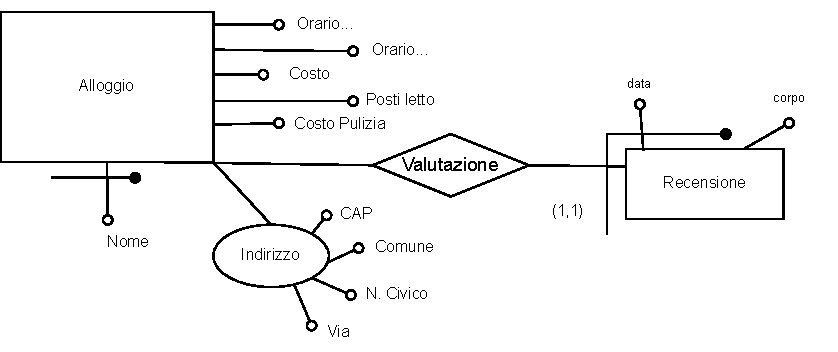
\includegraphics[width=\textwidth]{resources/page5.pdf}

\subsubsection{todo:titoletto}
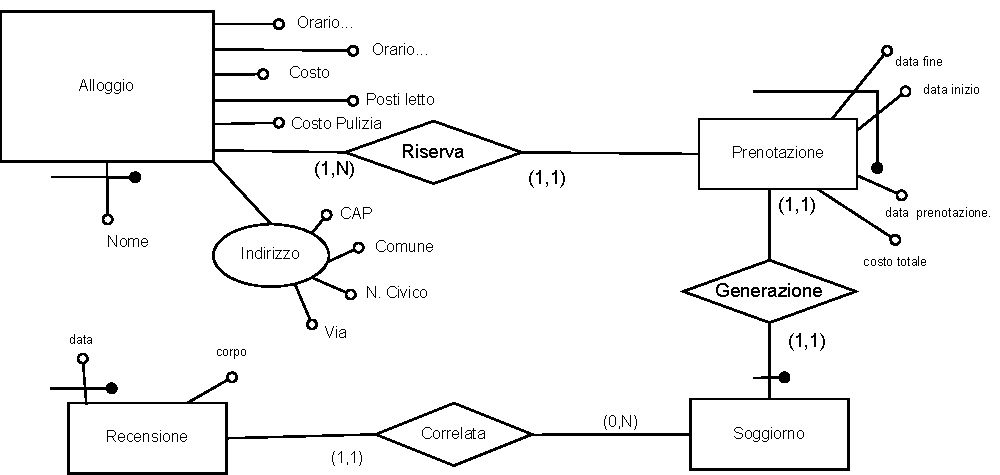
\includegraphics[width=\textwidth]{resources/page6.pdf}

\subsubsection{Tavola degli accessi}
Analizziamo l'operazione "\textbf{Scrittura di una recensione su un alloggio (3000 volte al giorno)}"

\small
\setlength\extrarowheight{2pt}
\begin{longtable}{|lccc|}
    \caption*{In presenza di ridondanza}                                             \\

    \hline \textbf{Concetto} & \textbf{Costrutto} & \textbf{Accessi} & \textbf{Tipo} \\\hline
    \endfirsthead

    \hline \textbf{Concetto} & \textbf{Costrutto} & \textbf{Accessi} & \textbf{Tipo} \\\hline
    \endhead

    \hline \multicolumn{4}{|r|}{{Continua all pagina successiva}}                    \\\hline
    \endfoot

    \hline
    \endlastfoot
    Alloggio                 & E                  & 1                & S             \\%\hline
    Alloggio                 & E                  & 1                & L             \\%\hline
    Recensione               & E                  & 1                & S             \\%\hline
    Valutazione              & R                  & 1                & S             \\%\hline
\end{longtable}
\normalsize

\small
\setlength\extrarowheight{2pt}
\begin{longtable}{|lccc|}
    \caption*{In presenza di ridondanza}                                             \\

    \hline \textbf{Concetto} & \textbf{Costrutto} & \textbf{Accessi} & \textbf{Tipo} \\\hline
    \endfirsthead

    \hline \textbf{Concetto} & \textbf{Costrutto} & \textbf{Accessi} & \textbf{Tipo} \\\hline
    \endhead

    \hline \multicolumn{4}{|r|}{{Continua all pagina successiva}}                    \\\hline
    \endfoot

    \hline
    \endlastfoot
    Alloggio                 & E                  & 1                & L             \\%\hline
    Riserva                  & R                  & 1                & L             \\%\hline
    Prenotazione             & E                  & 1                & L             \\%\hline
    Generazione              & R                  & 1                & L             \\%\hline
    Soggiorno                & E                  & 1                & S             \\%\hline
    Soggiorno                & E                  & 1                & L             \\%\hline
    Correlazione             & R                  & 1                & S             \\%\hline
    Recensione               & E                  & 1                & S             \\%\hline
\end{longtable}
\normalsize

Analisi di complessità in presenza di ridondanza:
\begin{itemize}
    \item In termini di tempo, vegnono effettuati un accesso in lettura e tre accessi in scrittura, quindi 3000 + 3000 * 3 * 2 (contiamo doppi gli accessi in scrittura), per un totale di 21 mila accessi.
    \item In termini di spazio, viene aggiunta una relazione in cui si memorizzano i dati chiave dell'alloggio all'interno dell'entità recensione: ipotizziamo quindi 200 byte per ogni recensione scritta.
          Considerando 200 byte per 2.000.000 di recensioni totali, il costo totale in termini di spazio risulta essere 200 * 2.000.000 (~381.47Mb).
\end{itemize}

Analisi di complessità in assenza di ridondanza:
\begin{itemize}
    \item In In termini di spazio, il costo totale è 0 byte.
    \item In termini di tempo, vegnono effettuati tre accessi in scrittura e cinque accessi in lettura, quindi 3000 * 5 + 3000 * 3 * 2 (contiamo doppi gli accessi in scrittura), per un totale di 33 mila accessi.
\end{itemize}

Dall'analisi effettuata, con l'assenza di ridondanza, risulta un peggioramento nei tempi di accesso (circa il 35\% di tempo in più) ma un risparmio notevole in termini di spreco di memoria: decidiamo per cui di rimuovere la ridondanza.

\subsection{Eliminazione delle generalizzazioni}
\subsubsection{Entità RECENSIONE}
\includegraphics[width=\textwidth]{resources/page7}
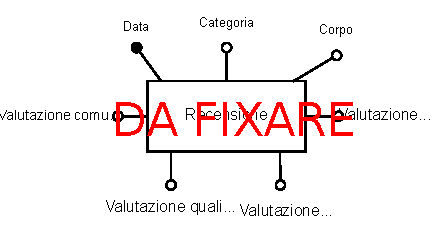
\includegraphics[width=\textwidth]{resources/page8}
La generalizzazione è di tipo totale ed esclusiva.\\
La decisione consiste nel raggruppamento delle entità	figlie nell'attributo categoria. Gli attributi specifici delle entità figlie (valutazioni) vengono spostate nell'entità padre, diventando annullabili. L'attributo categoria sarà un valore not null.

\subsubsection{Entità ALLOGGIO}
\includegraphics[width=\textwidth]{resources/page9}
\clearpage
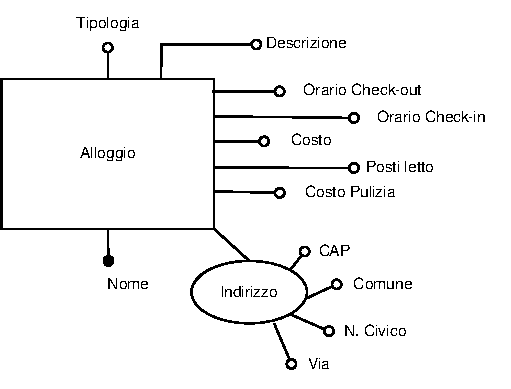
\includegraphics[width=\textwidth]{resources/page10}
La generalizzazione è di tipo totale ed esclusiva. La decisione consiste nel raggruppamento delle entità	figlie nell'attributo tipologia, con valore not null.

\subsubsection{Entità UTENTE}
\includegraphics[width=\textwidth]{resources/page11}
\includegraphics[width=\textwidth]{resources/page12}
La generalizzazione è di tipo totale ed esclusiva. La decisione consiste nel raggruppamento dell'entità figlia nell'attributo host, con valore not null. L'attributo superhost dell'entità figlia viene trasferito al padre.

\subsection{Partizionamento/accorpamento di entità e associazioni}
\includegraphics[width=\textwidth]{resources/page13}
\includegraphics[width=\textwidth]{resources/page14}
La decisione di accorpare le entità PRENOTAZIONE e SOGGIORNO in un'unica entità con attributo soggiorno (di tipo booleano) deriva dal fatto che l'entità SOGGIORNO viene generata dalle prenotazioni con stato "confermata".

{todo:immagine utente to Telefono}
Decidiamo di partizionare l'entità UTENTE estraendo l'attributo telefono e facendolo diventare una nuova entità TELEFONO, associata a UTENTE tramite la relazione POSSEDIMENTO.
{todo:immagine utente to Pagamento}
Decidiamo di partizionare l'entità UTENTE estraendo l'attributo Pagamento e facendolo diventare una nuova entità METODO DI PAGAMENTO, associata a UTENTE tramite la relazione APPARTENENZA.


\subsection{Eliminazione degli attributi composti}
L’attributo composto “\textbf{indirizzo}” viene eliminato seguendo la soluzione seguente: eliminare l’attributo composto e considerare i suoi componenti come attributi semplici. Nel caso di indirizzo abbiamo: via, numero civico e cap e comune.
Tale eliminazione viene effettuato nell'entità \textbf{ALLOGGIO}


\subsection{SCHEMA RELAZIONALE}
\begin{itemize}
  \item Utente (\underline{Email}, Nome, Cognome, Password, Host, Superhost)
  \item Alloggio (\underline{ID Alloggio}, Nome, Host, tipologia, Orario check-in, Orario check-out, Costo, Costo pulizia, Posti letto, CAP, Comune, Civico, Via)
        Alloggio (Host) referenzia Utente (Email)
  \item Prenotazione (\underline{ID Prenotazione}, Richiedente, ID Alloggio, Data inizio, Data fine, Soggiorno, Stato)
        Prenotazione (ID Alloggio) referenzia Alloggio (ID Alloggio)
        Prenotazione (Richiedente) referenzia Utente (Email)
  \item Recensione (\underline{ID Recensione}, Autore, ID Prenotazione, Data, Valutazione posizione, Valutazione pulizia, Valutazione qualità-prezzo, Valutazione comunicazione, Corpo)
        Prenotazione (Autore) referenzia Utente (Email)
        Prenotazione (ID Prenotazione) referenzia Prenotazione (ID Prenotazione)
  \item Commento (\underline{ ID Commento }, Data, ID Recensione, Autore, Corpo)
        Commento (Autore) referenzia Utente (Email)
        Commento (ID Recensione) referenzia Recensione (ID Recensione)
  \item Lista (\underline{ ID Lista }, Nome, Descrizione, Autore)
        Lista (Autore) referenzia Utente (Email)
  \item Contenuto(\underline{ ID Lista }, \underline{ID Alloggio})
        Contenuto (ID Lista) referenzia Lista (ID Lista)
        Contenuto (ID Alloggio) referenzia Alloggio (ID Alloggio)
\end{itemize}


% \subsection{SCHEMA RELAZIONALE}
% \begin{itemize}
%   \item Utente (\underline{Email}, Nome, Cognome, Password, Host, Superhost)
%   \item Alloggio (\underline{Nome},\underline{Host}, tipologia, Orario check-in, Orario check-out, Costo, Costo pulizia, Posti letto, CAP, Comune, Civico, Via)
%         Alloggio (Host) referenzia Utente (Email)
%   \item Prenotazione (\underline{Data inizio}, \underline{Data fine}, \underline{Nome alloggio}, \underline{Host alloggio}, \underline{Richiedente}, Soggiorno, Stato)
%         Prenotazione (Richiedente) referenzia Utente (Email)
%         Prenotazione (Nome alloggio, Host alloggio) referenzia Alloggio (Nome, Host)
%   \item Recensione (\underline{ Data }, \underline{ Data inizio prenotazione }, \underline{ Data fine prenotazione }, \underline{ Nome alloggio }, \underline{ Host alloggio }, \underline{ Richiedente prenotazione }, \underline{ Autore }, Valutazione posizione, Valutazione pulizia, Valutazione qualità-prezzo, Valutazione comunicazione, Corpo)
%         Recensione (Data inizio prenotazione, Data fine prenotazione, Nome alloggio, Host alloggio, Richiedente prenotazione) referenzia Prenotazione (Data inizio, Data fine, Nome alloggio, Host alloggio, Richiedente)
%         Recensione (Autore) referenzia Utente (Email)
%   \item Commento (\underline{ Data }, )   
%   \item Lista  
%   \item Servizio 
%   \item Richiesta
%   \item Generazione 
%   \item Elaborazione
%   \item Contenuto
%   \item Creazione
%   \item Scritto    
%   \item Correlazione 
%   \item Offerto     
%   \item Valutazione
% \end{itemize}


% \subsection{Analisi delle Ridondanze}
% \subsection{Eliminazione delle Generalizzazioni}
% \subsection{Partizionamento/Accorpamento di entità e associazioni}
% \subsection{Eventuale scelta degli identificatori principali}

\section{Schema E-R ristrutturato + Business Rules}
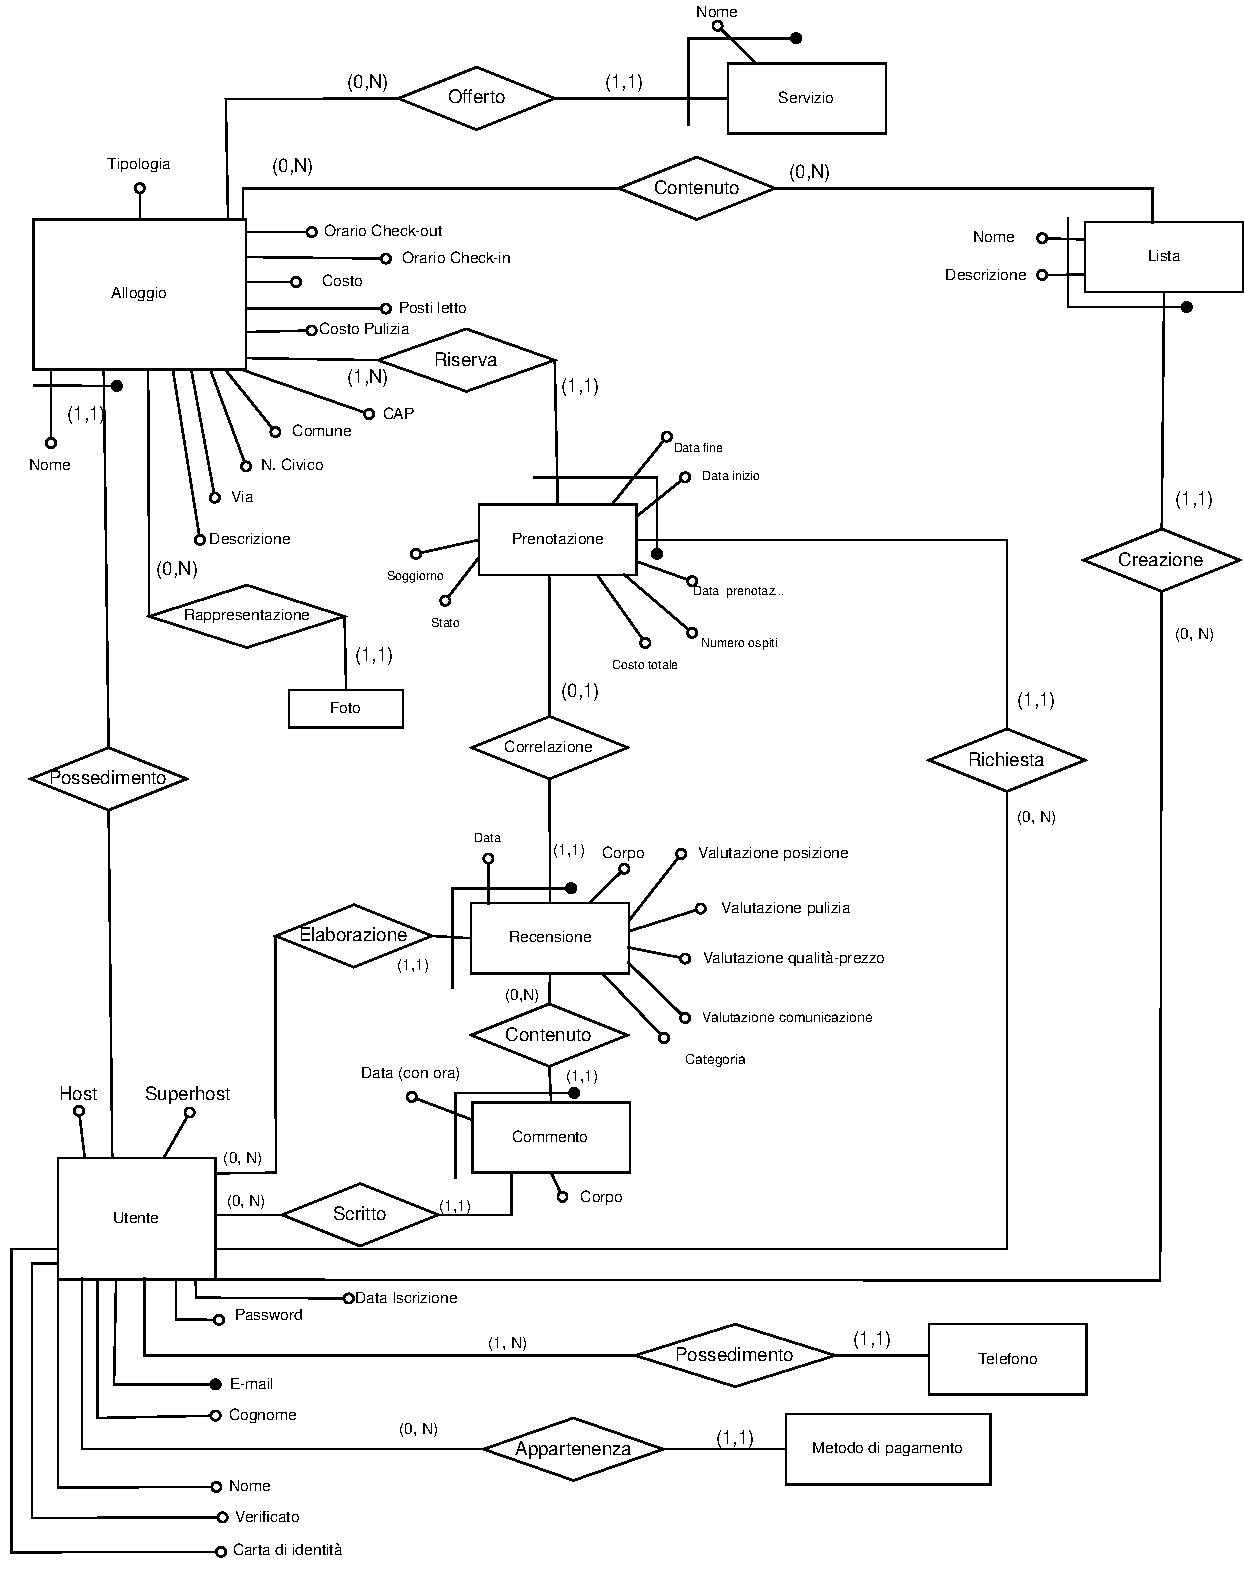
\includegraphics[width=\textwidth]{resources/pdf/ER-Ristrutturato.pdf}
\clearpage
\subsection{Business Rules}
\subsubsection{Derivate dal testo}
\begin{itemize}
  \item Un utente non può prenotare se non ha inserito un metodo di pagamento valido
  \item Un host per diventare superhost deve aver completato almeno 10 soggiorni per un totale di almeno 100 notti, aver conservato un tasso di cancellazione dell'1\% e avere una valutazione complessiva di 4.8 
  \item Un utente può visualizzare l'indirizzo di un alloggio solamente dopo aver effettuato una prenotazione con avvenuta conferma da parte dell'host
  \item Un utente non può indicare in una prenotazione nomi di altri ospiti, se questi non sono iscritti alla piattaforma 
  \item Un utente può valutare un host, e viceversa, solamente al termine del soggiorno soggetto alla valutazione
  \item Un utente non può cancellare una prenotazione dopo l'inizio di un soggiorno
  \item Un host non può cancellare una prenotazione dopo l'inizio di un soggiorno
  \item Una recensione da parte di un host risulta visibile solamente quando il soggiorno a cui fa riferimento riceve la recensione da parte dell'utente, e viceversa
  \item Una recensione risulta visibile trascorsi 7 giorni dal termine del soggiorno a cui fa riferimento
  \item Le recensioni sono visibili sui profili degli utenti suddivise in base a quelle ricevute come ospite e come host
\end{itemize}

\subsubsection{Introdotte}
\begin{itemize}
  
  \item L'indirizzo e-mail di un utente che effettua la registrazione deve corrispondere al formato e-mail (nomemail@dominio.TLD)
  \item Un utente viene ritenuto host se possiede almeno un alloggio
  \item Un utente può cancellare solamente le proprie prenotazioni effettuate
  \item Un host può confermare o rifiutare solamente le prenotazioni effettuate ai propri alloggi
  \item Le cancellazioni delle prenotazioni da parte degli utenti non influisce sul tasso di cancellazione di un host
  \item Un utente non può indicare, in una prenotazione, un numero di ospiti maggiore dei posti disponibili nell'alloggio prenotato
  \item Un utente non può effettuare una prenotazione presso un alloggio di tipo stanza condivisa se il numero di posti letto ancora disponibili non è sufficiente
  \item Un utente non può valutare soggiorni non prenotati da lui
  \item Un host non può valutare ospiti che non hanno effettuato soggiorni presso i proprio alloggi
  \item Un utente non può scrivere commenti sotto recensioni altrui
  \item Un host non può scrivere commenti sotto recensioni altrui
  \item Un utente non può effettuare due recensioni per lo stesso soggiorno
  \item Una prenotazione non può essere effettuata presso un alloggio di tipo stanza singola o appartamento se la data di inizio o di fine intercorre tra la data di inizio e di fine di un'altra prenotazione presso lo stesso alloggio
  \item Una prenotazione non può essere cancellata completamente dal sistema: quando una prenotazione viene cancellata, viene aggiornato il suo stato a "cancellata"
  \item Una prenotazione non può essere cancellata se la data di inizio è antecedente alla data odata di oggi
  \item Quando un alloggio viene rimosso, lo stato delle sue prenotazioni con soggiorno false viene aggiornato a "cancellata"
  \item Quando un host viene cancellato, lo stato delle prenotazioni in corso associate ai suoi alloggi viene aggiornato a "cancellata"
  \item Quando un utente viene cancellato, le recensioni effettuate risulteranno scritte da "utenti cancellato"
\end{itemize}

\clearpage
\section{Schema Relazionale}
\begin{itemize}
    \item Utente (\underline{Email}, Nome, Cognome, Password, Host, Superhost, Verificato, Carta di identità)
    \item Telefono (\underline{Utente}, \underline{Numero}, Prefisso)
    \item Pagamento (\underline{Utente}, \underline{Numero}, Circuito)
    \item Utente (\underline{Email}, Nome, Cognome, Password, Host, Superhost)
    \item Alloggio (\underline{ID Alloggio}, Nome, Host, Descrizione, Tipologia, Orario check-in, Orario check-out, Costo, Costo pulizia, Posti letto, CAP, Comune, Civico, Via)
          Alloggio (Host) referenzia Utente (Email)
    \item Foto (\underline{Path}, \underline{Alloggio})
          Alloggio (Foto) referenzia Alloggio (ID Alloggio)
    \item Prenotazione (\underline{ID Prenotazione}, Richiedente, ID Alloggio, Data inizio, Data fine, Soggiorno, Stato, Numero ospiti)
          Prenotazione (ID Alloggio) referenzia Alloggio (ID Alloggio)
          Prenotazione (Richiedente) referenzia Utente (Email)
    \item Recensione (\underline{ID Recensione}, Autore, ID Prenotazione, Data, Categoria, Valutazione posizione, Valutazione pulizia, Valutazione qualità-prezzo, Valutazione comunicazione, Corpo)
          Recensione (Autore) referenzia Utente (Email)
          Recensione (ID Prenotazione) referenzia Prenotazione (ID Prenotazione)
    \item Commento (\underline{ ID Commento }, Data, ID Recensione, Autore, Corpo)
          Commento (Autore) referenzia Utente (Email)
          Commento (ID Recensione) referenzia Recensione (ID Recensione)
    \item Lista (\underline{ ID Lista }, Nome, Descrizione, Autore)
          Lista (Autore) referenzia Utente (Email)
    \item Contenuto(\underline{ ID Lista }, \underline{ID Alloggio})
          Contenuto (ID Lista) referenzia Lista (ID Lista)
          Contenuto (ID Alloggio) referenzia Alloggio (ID Alloggio)
\end{itemize}

\chapter{Implementazione}

Riportiamo in seguito alcune query significative per il nostro database

\section{DDL di Creazione dei Database}
\lstinputlisting{../sql/DDL/db_init.sql}
\clearpage
\lstinputlisting{../sql/DDL/1.sql}
\lstinputlisting{../sql/DDL/2.sql}
\lstinputlisting{../sql/DDL/3.sql}
\clearpage
\lstinputlisting{../sql/DDL/4.sql}
\lstinputlisting{../sql/DDL/5.sql}
\clearpage
\lstinputlisting{../sql/DDL/6.sql}
\clearpage
\lstinputlisting{../sql/DDL/7.sql}
\lstinputlisting{../sql/DDL/8.sql}
\lstinputlisting{../sql/DDL/9.sql}
\lstinputlisting{../sql/DDL/10.sql}
\lstinputlisting{../sql/DDL/11.sql}

\clearpage
\section{DML di Popolamento di Tutte le Tabelle del Database}
\lstinputlisting{../sql/DML/dummy_data.sql}

\clearpage
\section{Qualche Operazione di cancellazione e modifica}
\lstinputlisting{../sql/DML/crud_data.sql}

\subsection{Qualche operazione di sistema}
\lstinputlisting{../sql/DML/operation.sql}

\end{document}